\begin{figure}[H]
\centering
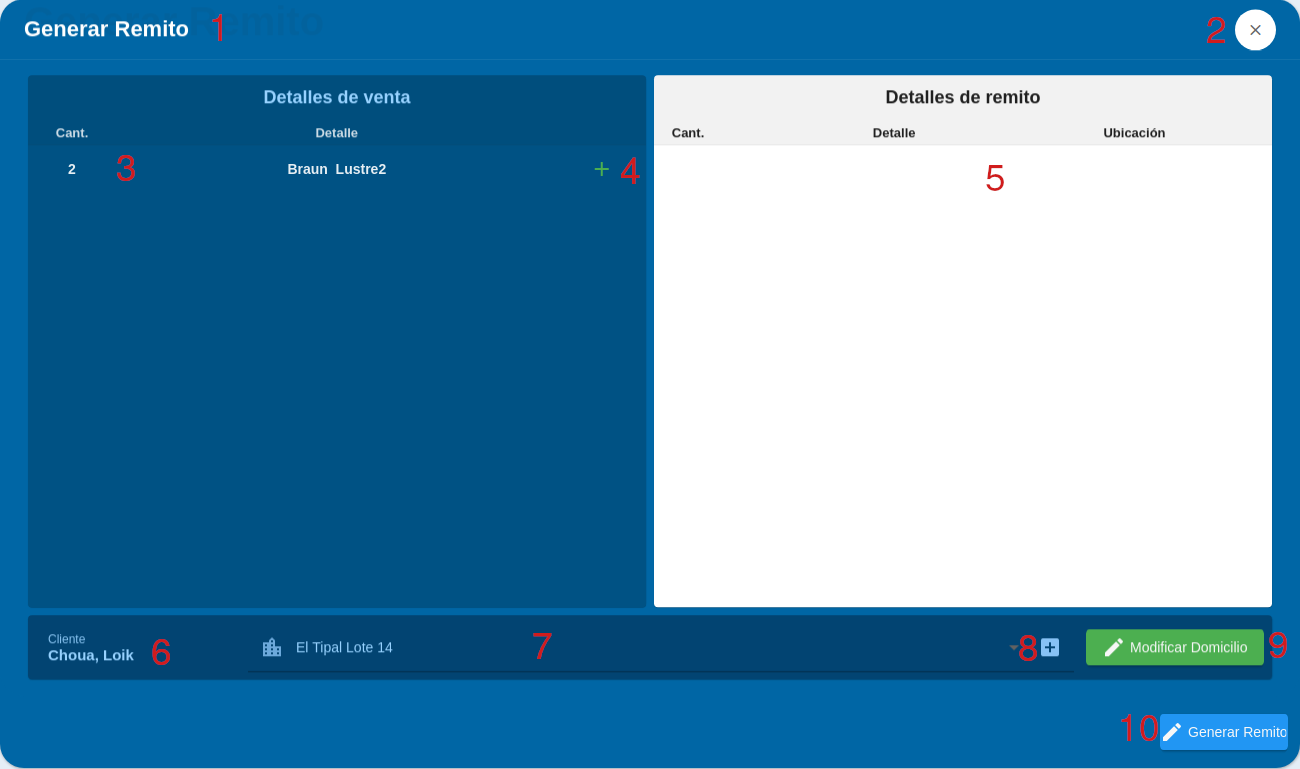
\includegraphics[width=\textwidth,height=\textheight,keepaspectratio]{Escenarios/AD-21-00}
\caption{Escenario - AD-21-00}
\label{fig:AD-21-00}
\end{figure}
Este escenario permite a los usuarios generar un remito a partir de una venta. El campo \textbf{AD-21-01} indica la operación a realizarse. Con el botón \textbf{AD-21-02} se podrá cerrar la ventana y volver al escenario \textbf{AD-10-00}. 
En la sección \textbf{AD-21-03} se mostrarán todas las lineas de venta de la venta seleccionada. Un click \textbf{AD-21-04}, agregará a la linea de venta a las elegidas para crear el remito. En la sección \textbf{AD-21-05} se mostrarán todas las lineas de venta seleccionadas para crear el remito.
En el campo \textbf{AD-21-06} se mostrará el nombre cliente, y en la lista desplegable \textbf{AD-21-07} se podrá elegir un domicilio del cliente para crear el remito. Un click en botón \textbf{AD-21-08} navegará al escenario \textbf{AD-31-00} que le permite al usuario crear un nuevo domicilio para el cliente. Un click en botón \textbf{AD-21-09} actualizará el domicilio del cliente para crear el domicilio.
Un click en el botón \textbf{AD-21-10} creará el remito y navegará al escenario \textbf{AD-16-00}.
\\
